\chapter{Application Flow Monitoring}

\begin{chapintro}

Deep packet inspection (DPI) and IP flow monitoring are frequently used network monitoring approaches nowadays. Although the DPI provides application visibility, detailed examination of every packet is computationally intensive. The IP flow monitoring achieves high performance by processing only packet headers, but provides no details about the traffic content. Application flow monitoring is proposed as an attempt to combine DPI accuracy and IP flow monitoring performance. This chapter ... 
% contributions

% Petr Velan and Pavel Čeleda. “Next Generation Application-Aware Flow Monitoring” - related but cannot be directly included.
% Petr Velan, Tomáš Jirsík, and Pavel Čeleda. “Design and Evaluation of HTTP Protocol Parsers for IPFIX Measurement”
The papers related to this chapter are~\cite{Velan-2014-Next, Velan-2013-Design}.

The organisation of this chapter is as follows:
\begin{itemize}
  \item Section~\ref{sec:creating-application-flow} 
  \item Section~\ref{sec:http-parser-design}
  \item Section~\ref{sec:app-conclusions} concludes the chapter.
\end{itemize}

\end{chapintro}

\newpage


\section{Motivation}
The number of different applications communicating over the Internet is ever increasing and so is the need for application-aware network monitoring. However, building network monitoring systems is always a compromise between accuracy and performance. The more information processed, the more accurate the monitoring system is. Unfortunately, thorough examination of the traffic is computationally expensive~\cite{Gao-2006-Efficient, Lai-2004-Parallel}. Application flow monitoring is a network monitoring approach created to exploit the benefits of deep packet inspection (DPI). Integration of the DPI into flow monitoring allows for information aggregation, which provides better performance than the DPI alone.

Application flow monitoring is a subset of flow monitoring as described in the Chapter~\ref{chap:network-flow-monitoring} and all provided definitions hold for it as well. The reason to treat application flow monitoring as a special case is that processing application layer introduces specific issues which require special attention. Therefore, we distinguish IP flow monitoring (flow keys and values of other properties  are extracted only from link, network, and transport layer headers) and application flow monitoring as two distinct part of flow monitoring.

The application flow monitoring usually utilizes two main concepts: application identification (also known as traffic classification) and application visibility. The application identification allows to recognize the application protocol of a particular flow. The type of application is usually added as a single field to the exported flow record. The application visibility provides more information about the information carried by the application protocol itself. Application identification is a prerequisite of the application visibility. However, application identification can be done with use of machine learning techniques even without observing packet payloads.

This chapter describes the differences between IP flow monitoring and application flow monitoring that have to be taken into consideration when the application flow monitoring process is designed and deployed. The most important part of application visibility is the design of application parsers. To illustrate the complexity of the application parser design, we propose and discuss several designs of HTTP protocol parsers at the end of this chapter.

The benefits of application flow monitoring are discussed extensively in the Chapter~\ref{chap:traffic-analysis-using-application-flow-monitoring}.

\section{Related Work}

The use of machine learning techniques for traffic classification has attracted many researchers~\cite{Nguyen-2008-Survey, Dainotti-2012-Issues, Finsterbusch-2014-Survey}. A complete survey of the used techniques and results is out of scope of this work, however, the methods of application identification for encrypted traffic are surveyed in the Chapter~\ref{chap:measurement-of-encrypted-traffic}.

\subsection{Application Parsers}
Although application visibility is provided by a variety of commercial products such as dedicated probes, forwarding devices, and firewalls, it does not seem to be as attractive research topic as application identification. However, significant research effort was invested in automating the creation of application parsers. \citeauthor{Pang-2006-binpac} created a language and accompanying parser called \emph{binpac}~\cite{Pang-2006-binpac} in \citeyear{Pang-2006-binpac}. It allows to generate application parsers from their declarative description. A slightly different approach was taken by \citeauthor{Caballero-2007-Polyglot} in \citeyear{Caballero-2007-Polyglot}. The authors created a tool called \emph{Polygot}~\cite{Caballero-2007-Polyglot} which is used to reverse engineer application protocol headers. Similar work was published at the same time by \citeauthor{Cui-2007-Discoverer} in \cite{Cui-2007-Discoverer}. They presented a tool called \emph{Discoverer} that could automatically reverse engineering the protocol message formats of an application from its network trace. \citeauthor{Davidson-2009-Protocol} introduce a notion of using a higher order attribute grammar in~\cite{Davidson-2009-Protocol}, which allows to describe the structure of application protocols for which the use of context-free grammar is impractical or impossible. Another framework, called \emph{Spicy}~\cite{Sommer-2016-Spicy} was introduced by \citeauthor{Sommer-2016-Spicy}. It consists of format specification language, compiler toolchain and an API for DPI applications which allows for easy integration of the generated parsers to existing tools.

\subsection{Application Flow Exporters}
There is a number of open-source tools and commercial products that support an export of flows including application information. Most of them already support the IPFIX protocol for the encoding of application information~\cite{Hofstede-2014-Flow}, however, there are still a few that add custom elements to the NetFlow v9 protocol, which can cause element collisions and compatibility problems. Table~\ref{tab:flow-exporters} shows an overview of the flow exporters discussed in this section.

\begin{table}[ht!]
    \centering
    \footnotesize
    \renewcommand{\arraystretch}{1.2}
    \begin{tabular}{>{\centering}m{1.5cm}| >{\centering}m{2cm} |c|>{\centering}m{0.8cm}|>{\centering\arraybackslash}m{5.1cm}}
    \toprule
    \textbf{Vendor}    & \textbf{Product}                   & \textbf{IPFIX} & \textbf{App. ident.} & \textbf{App. visibility}  \\ \hline
    CERT NetSA         & YAF                                & \cmark         & \cmark                       & FTP, HTTP, IMAP, RTSP, SIP, SMTP, SSH, DNS, SSL/TLS, IRC, NNTP, POP3, SLP, TFTP, MySQL, DNP3, Modbus and RTP \\ \hline
    ntop               & nProbe                             & \cmark         & \cmark                       & \\ \hline
    ntop               & nProbe Pro                         & \cmark         & \cmark                       & HTTP, DHCP, DNS, MySQL, Oracle DB, BGP, IMAP, POP3, SMTP, Radius, Diameter, GTP, S1AP, SSDP, NetBIOS  \\ \hline
    FlowMon Networks   & Flowmon Probe                      & \cmark         & \cmark                       & HTTP, DNS, DHCP, SMB, E-mail, MSSQL, VoIP SIP and other protocols \\ \hline
    Cisco              & Application Visibility and Control & \cmark         & \cmark                       & \\ \hline
    Lancope            & Stealthwatch FlowSensor            & \cmark         & \cmark                       & \\ \hline
    Palo Alto Networks & Next-Generation Firewall           &                & \cmark                       & \\ \bottomrule
    \end{tabular}
    \caption{Flow Exporters Supporting Application Flow Monitoring}
    \label{tab:flow-exporters}
\end{table}

% TODO mention performance: throughput depends on packet size and used application identification and visibility plugins, incomparable

Two open-source flow exporters pioneer the application flow monitoring: YAF and nProbe. YAF (Yet Another Flowmeter)~\cite{Inacio-2010-YAF} was created as a reference implementation of a flow exporter conforming to the IPFIX standard. YAF supports custom rules for application identification~\cite{CERTNSAGET--yaf}. It can match applications by regular expressions in combination with ports, by signatures or by using dynamically loaded plugins for processing packet payloads. Application visibility~\cite{ESCERTNSAGET--yaf} is supported for flows where application identification succeeded. YAF allows to load plugins that perform the DPI and export the optional information elements using a subTemplateMultiList feature of the IPFIX protocol.Application protocols supported according to the YAF documentation are listed in the Table~\ref{tab:flow-exporters}.

The nProbe~\cite{Deri-2003-nProbe} is a flow probe created by \citeauthor{Deri-2003-nProbe} and published in~\citeyear{Deri-2003-nProbe}. Although the nProbe is both flow exporter and flow collector, we focus only on its features as an exporter. Application identification was added to nProbe in 2011~\cite{ntop-2011-Unveiling}. It is based on the OpenDPI open-source traffic identification library, however, the authors of nProbe improved the library and showed that their version (nDPI) can be used for high-speed traffic identification~\cite{Deri-2014-nDPI}. The nProbe supports custom flow record export format for NetFlow v9 and IPFIX protocols. The user us allowed to configure her own list of templates that is used to transport data to a flow collector. Support for application visibility is provided by the use of optional plugins. However, these plugins are not available for the open-source version of nProbe and can only be used with nProbe Pro version.

There are several available probes, forwarding devices, and firewalls that support at least limited application flow monitoring. It is often difficult or impossible to gain detailed information about the level of application identification and visibility supported by commercial devices. The information provided in the rest of this section is therefore only an overview of some of the available products from publicly obtainable information.

The nProbe Pro version is a commercial version of nProbe supporting plugins that provide application visibility. Application protocols supported according to the nProbe documentation are listed in the Table~\ref{tab:flow-exporters}.

Another flow monitoring probe is the Flowmon Probe~\cite{FlowmonNetworks--Flowmon} from Flowmon Networks. Support for application identification is provided using the libprotoident~\cite{Alcock-2012-libprotoident} library and application visibility is provided by multiple application processing plugins. The application visibility is independent of application identification, therefore each application processing plugin must have its own application identification algorithm for the supported application protocol. The Flomon Probe exports flow records using IPFIX protocol and the application fields are encoded using the Flowmon Networks Private Enterprise Number (PEN).

Cisco provides support for application identification both in forwarding devices as well as in dedicated probes called NetFlow Generation Appliances. The Cisco Application Visibility and Control (AVC)~\cite{CiscoSystems--Cisco} technology uses Network-Based Application Recognition 2 (NBAR2) Protocol Library~\cite{CiscoSystems--NBAR2} for application identification and NetFlow and IPFIX protocols for flow export. NBAR2 is a deep packet inspection library which uses signatures to classify traffic to categories and subcategories. No application visibility is supported by NBAR2, therefore no details from application protocol headers are exported by the AVC.

The Stealthwatch FlowSensor\cite{Lancope--Stealthwatch} is a flow monitoring probe by Lancope which supports application identification using DPI and behavioural analysis. The flow export using IPFIX protocol is supported as well as older NetFlow protocols.

An example of a firewall with limited application flow monitoring support is the Next-Generation Firewall from Palo Alto Networks~\cite{PAN--Next}. It supports application identification and can export application labels using NetFlow v9 protocol. Although the feature is called visibility and control, which is similar to the Cisco AVC, no application visibility apart from the identification is provided.

All presented flow exporters and flow monitoring devices struggle to achieve high throughput to be able to monitor high-speed networks. However, we avoided direct comparison of declared throughput of the flow probes as it highly depends on the nature of the traffic, supported application protocols and hardware configuration. More information about flow measurement in high-speed networks is provided in the Chapter~\ref{chap:flow-monitoring-performance}

\section{Application Flow Definition}
% application flow is a subset of flow as defined in chap 2.
% application flow definition (in text) 
% beware of application identification vs application visibility, it must fit the definition

% explain that aplication flow monitoring means that:
% - primary: information from application layer is added to flow records
% - secondary:
%  - application logic (not necessarily in L7) affect the flow creation process, e.g. monitoring of tunnels
%  - less typical but can also be considered as application flow monitoring: additional information can be added to flow records from external sources (geolocation)

\section{Creating Application Flow}\label{sec:creating-application-flow}
% 
% application flow monitoring changes to flow monitoring (sometimes called IP flow monitoring):
% - packet processing: 
%   - L7 parsing is sometimes complex -> section with Design of an HTTP Parser
%   - need to support recursion for tunnel monitoring
% - flow creation
%   - more complex flow keys
%   - split flows after application event (next request in a single connection (HTTP pipelining))
%   - retain application data for flows split by active timeout
%   - size of flow records -> large flow caches
% - flow export
%   - described in previous chapter - long flows, different semantics for new elements
%   - when URLs, domain names etc are exported in fixed lenght, the original length should be exported as well



\iinfo{Taken from: Application Flow Monitoring Challenges}

\itodo{TODO: vyporadat se s opakujicimi se hlavickami (HTTP), doplnit definici flow z predchozi kapitoly\\
- Flow expiration/termination vs app flow splitting}

The application flow monitoring is a complex process. Packets need to be received from the network, transported to computer memory (RAM), parsed, aggregated to flow records based on the parsed information, and exported to flow collectors for further processing. The process is depicted in Figure~\ref{fig:flow-exporter-schema}. This section describes the whole flow measurement process, points out where it is affected by the application processing and introduces some of the related challenges.

\begin{figure}[tb!]
  \begin{center}
    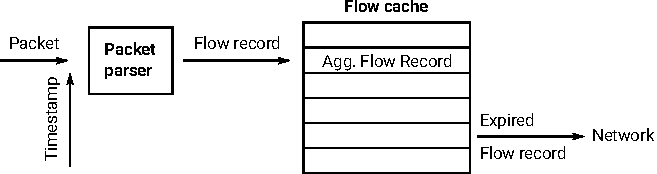
\includegraphics[width=\textwidth]{figures/flow-exporter-schema}
  \end{center}
  \caption{A Flow Exporter Schema}
  \label{fig:flow-exporter-schema}
\end{figure}


The packet reception is unchanged for application flow monitoring unless the NIC processes the application layer. This scenario is discussed later in Hardware Accelerated Techniques section.


\subsection{Packet Processing}

% \cite{Pang-2006-binpac}

The basic task of the packet parsing is to extract connection attributes such as IP addresses, transport protocol, and ports to determine which flow the packet belongs to. Moreover, it obtains additional information of interest, especially from application protocols. The parser must be resilient to malformed packets and unknown protocols while supporting a wide range of existing network and application protocols.

Link, network, and transport headers of IP packets follow a strictly defined structure so that the network devices such as routers can process the packets swiftly. However, application layer protocols often rely on connections being established between compatible endpoints. For this reason, application protocol identification is a difficult task. A lot of attention has been dedicated to research of application identification in network traffic in the past, for example in the work of \citeauthor{Bujlow-2015-classification}~\cite{Bujlow-2015-classification}, however, not every approach is suitable for the flow monitoring scenario.

With increasing deployment of encryption for all kinds of communication, the task of application flow monitoring becomes more difficult. Without access to application payload, the amount of information that can be extracted from the traffic is diminished. However, there are statistical and machine learning methods that are able to recognize specific applications even in encrypted traffic with high accuracy. Moreover, useful information such as a version of encryption protocol, certificates, or supported cipher suites, can be extracted from encrypted traffic. This information can be used to identify malicious encrypted traffic. The possibilities of processing and analysis of encrypted traffic were surveyed by the authors of~\cite{Velan-2015-Survey}.

\subsection{Flow Creation}

Application protocol measurement may require flow record to be expired early. For example, when HTTP protocol supports pipelining, multiple requests and responses can be carried out over a single connection. When it is desirable to keep track of each request/response pair, existing flow record might be exported when a new request is encountered on the same connection. Therefore, application flow monitoring  also affects the number of generated flow records, which needs to be taken into consideration during further processing of the flow records.

\iimprove{TODO: keeping application data from expired flow records (long HTTP video streaming)}

Another impact of the application flow monitoring on the flow aggregation is the increased size of flow records. The information extracted from application protocols can be quite large in comparison to network and transport layers lengths. While the typical IPv4 header length is 20 bytes, typical TCP header length is 32 bytes, the HTTP URL can easily be several hundred bytes long. Therefore, the length of flow records of application flow monitoring is several times larger than without the application layer. There are two main negative impacts of such large flow records. Firstly, the flow cache might require much more RAM than standard flow monitoring flow cache. Secondly, even if the cache fits into RAM, it degrades the performance of the memory accesses because data locality is decreased and a CPU experiences more cache misses. For these reasons, it must be carefully considered which information is placed in each flow record and how it is encoded.

\subsection{Flow Export}

Several issues might be encountered with flow export when application flow monitoring is applied. First, due to the larger amount of exported data, the link to a flow collector might be congested. We have experienced this issue when application flow records from a 10G link were exported simultaneously to several collectors over old 100\,Mb/s management interface. The solution is either to simply upgrade to 1\,Gb/s management interface or, better, to reduce the number of targets of the export and distribute the flows as necessary through replicating proxy in the location of the collectors. The latter solution saves network bandwidth used for monitoring purposes and should be preferred if possible.

Another issue that might be encountered due to large flow record is that single record might be larger than MTU of the management network interface on the flow exporting device. In such a case UDP transport protocol, which is still widely used for flow export, cannot be used without fragmenting IP packets. The fragmentation might cause a performance problem for the flow collector which has to reassemble the packets. It also increases the probability of data loss as single lost fragment invalidates the whole message.


\section{Common Issues} % what is specific to application protocols, otherwise it should be at the end of previous chapter

% shortening of string values - add some indication of shortening or original length

\section{Design of an HTTP Parser: A Study}\label{sec:http-parser-design} % put in Velan-2013-Design paper 

\section{Conclusions}\label{sec:app-conclusions}